\section{Outline of the Proposed Method}
\label{sec:outline}

Our approach relies on the well-known observation that the greater the similarity between two projections, the more likely they originated from two 3D particles that adopted close orientations in the ice layer prior to imaging\footnote{Up to some possible intrinsic symmetries of the objects, which are discussed later.}. This principle guides a number of applications in SPA, including that of projection matching~\cite{penczek1994ribosome}.

Taking this line of thought further, we train a function---parametrized as a neural network---to predict the relative orientation between two projections based on their similarity. To make such training possible, we capitalize on our ability to model the cryo-EM imaging procedure to generate a large, representative synthetic dataset using publicly available 3D atomic models.

Using this trained distance function, we can estimate the relative orientations between pairs of projections in any real dataset. Our postulate is that we can then recover, from these estimated relative orientations, the orientations themselves through an appropriate minimization scheme. This two-steps pipeline is illustrated in Figure~\ref{fig:overview-pipeline}. \\ 

% ---
\begin{figure}[h!]
    \center
    \fbox{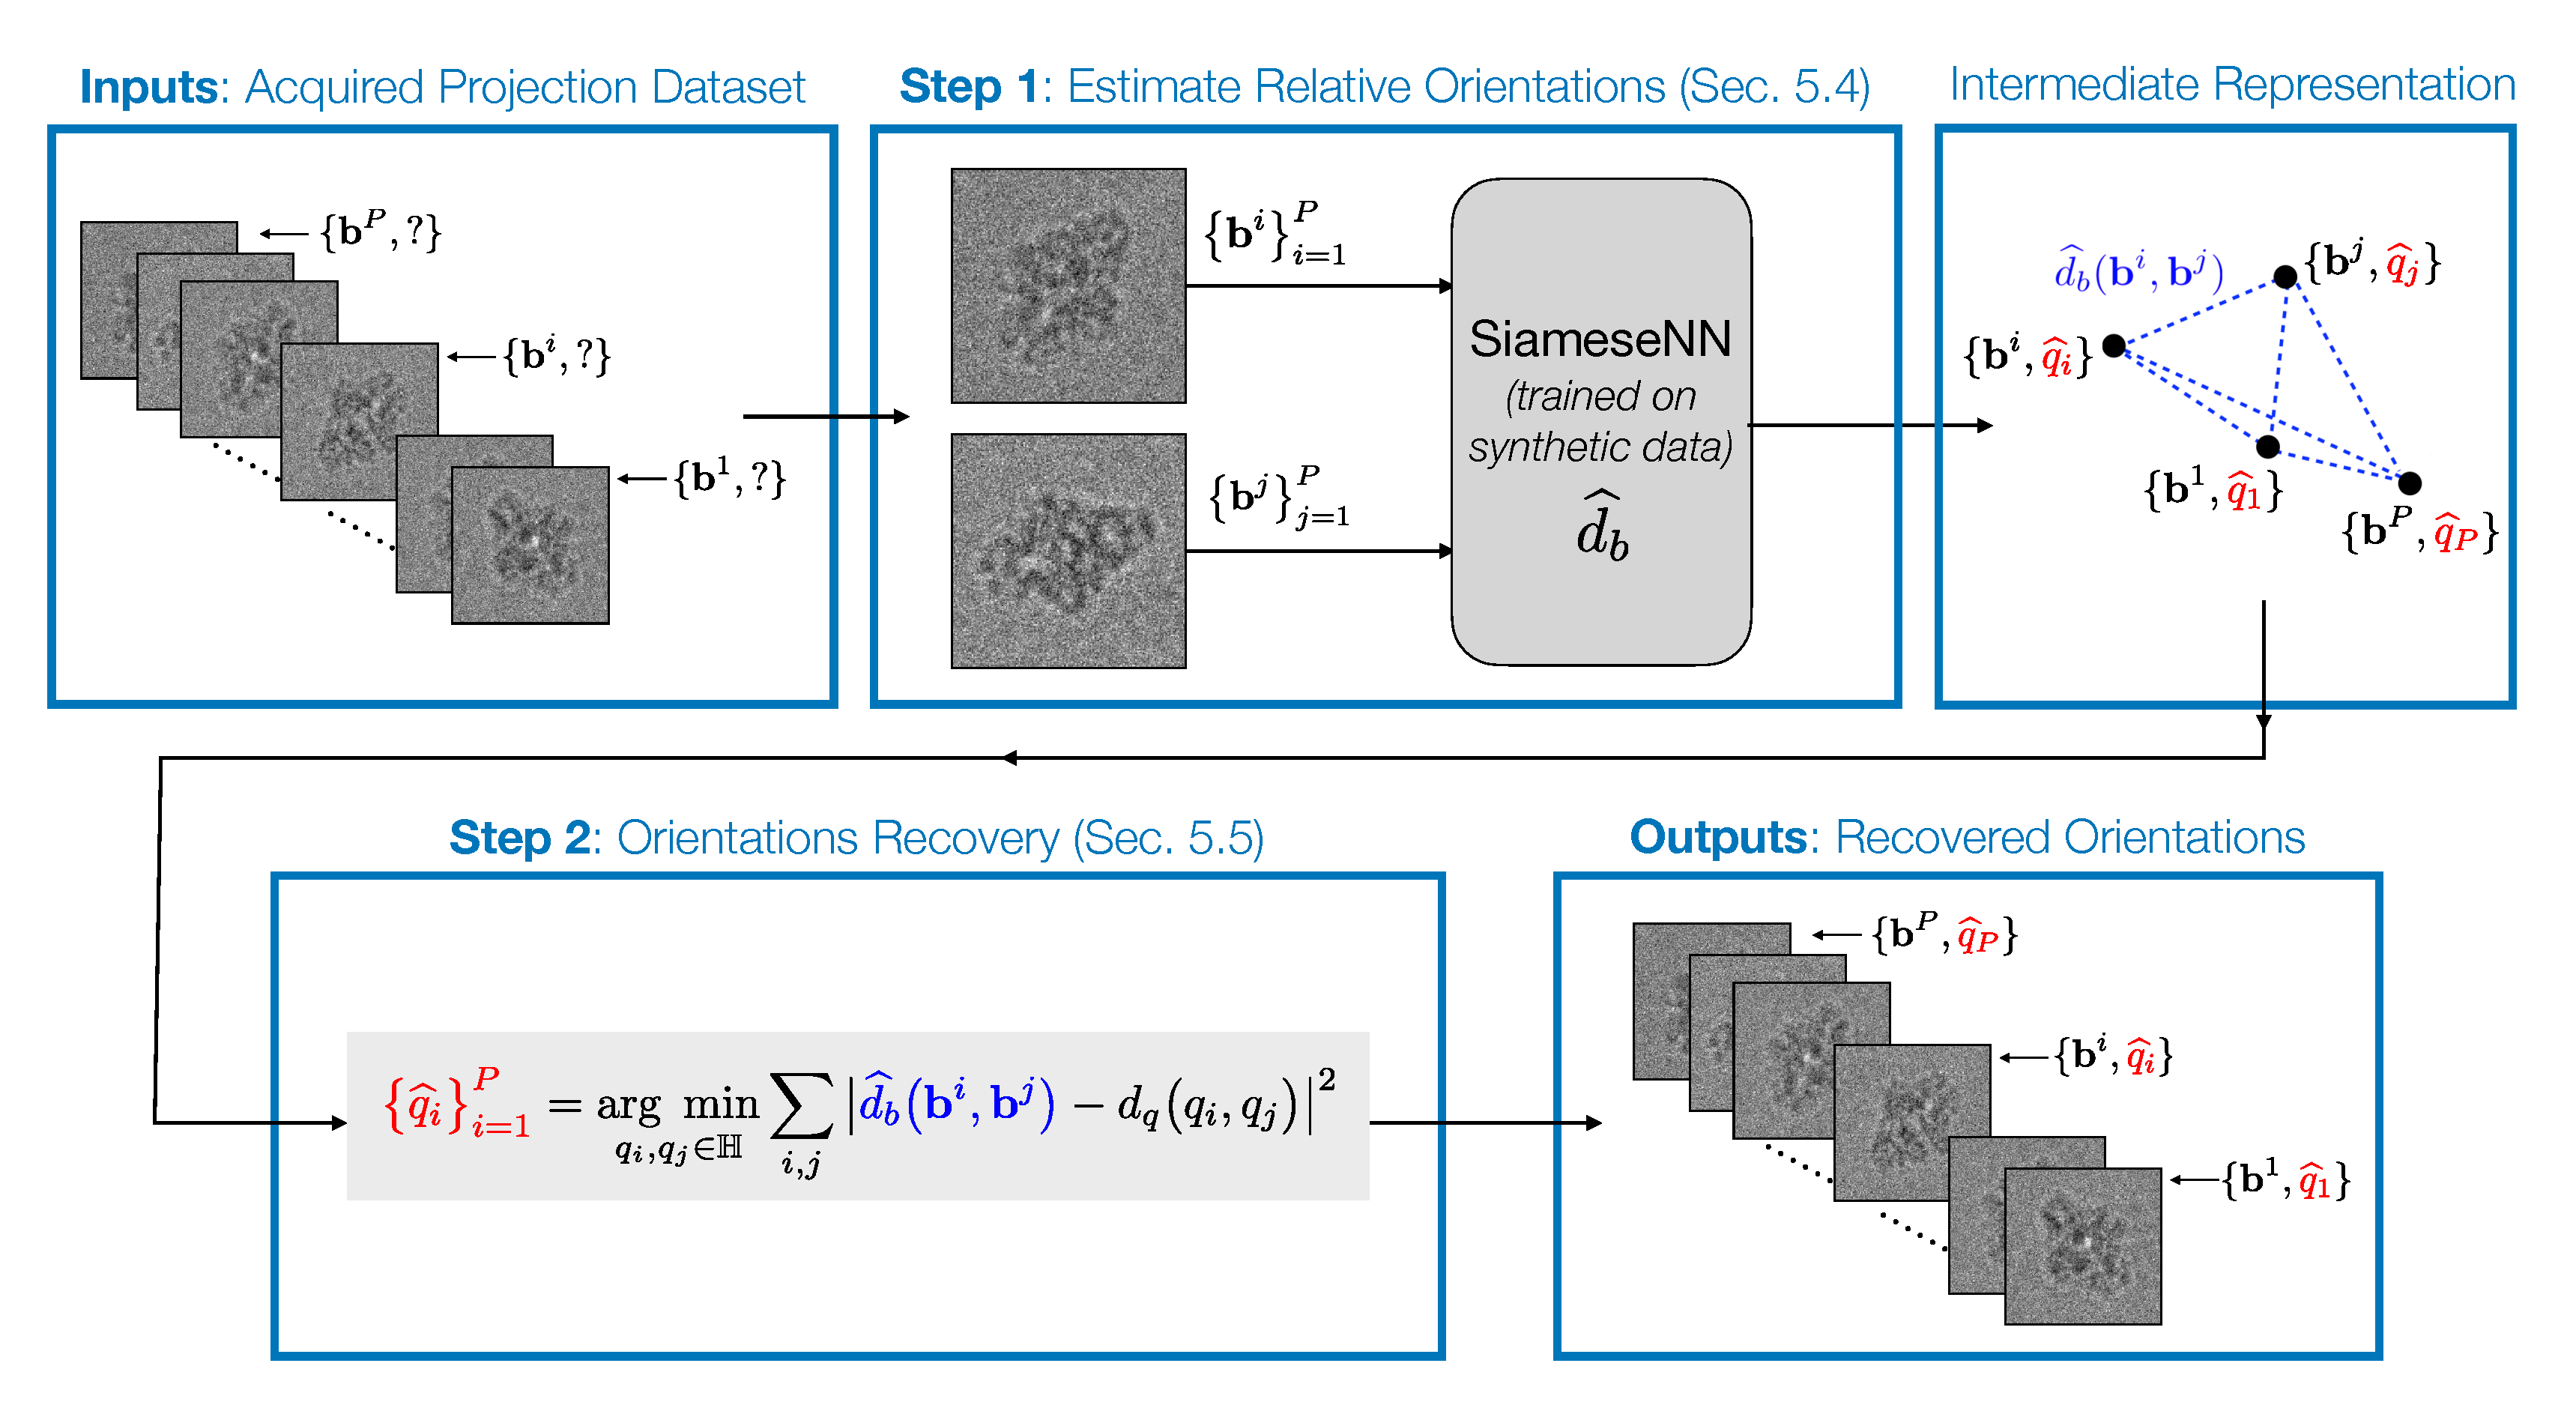
\includegraphics[width=\textwidth]{images/pipeline-overview.pdf}}
    \caption{Overview of the proposed two-steps method: 1) estimate the relative orientations between projection pairs through a learned distance $\widehat{d}_b$, and 2) recover the orientations from the estimated relative orientations. We denote a $p$th projection by $\mathbf{b}^p$ and its orientation by $q_p$. The geodesic distance between two orientations is denoted by $d_q$.}
    \label{fig:overview-pipeline}
\end{figure}
% ---

The task of recovering points based on their relative distances has been extensively studied in the literature, mostly within the framework of dimensionality reduction and primarily for the case of \textit{Euclidean} embedding spaces\footnote{An ``embedding space'' corresponds to the (often lower-dimensional) space in which data is embedded, \textit{i.e.}, mapped to in such a way that the relative distances between its points are preserved as much as possible.}~\cite{belkin2003laplacian,kruskal1978multidimensional, maaten2008visualizing, mcinnes2018umap,dokmanic2015euclidean} . In that respect, the short example given by Dokmanic \textit{et al.} in~\cite{dokmanic2015euclidean} efficiently illustrates the philosophy behind such methods (see the ``An Analogy'' box). \\

% ---------------------------------------------------
\setlength{\fboxsep}{1em}\noindent\fbox{\parbox{0.95\textwidth}{%
\textbf{An Analogy: Mapping the Position of Swiss Cities with a Train Timetable~\cite{dokmanic2015euclidean}} \\

% ---
\begin{wrapfigure}{r}{0.45\textwidth}
  \begin{center}
    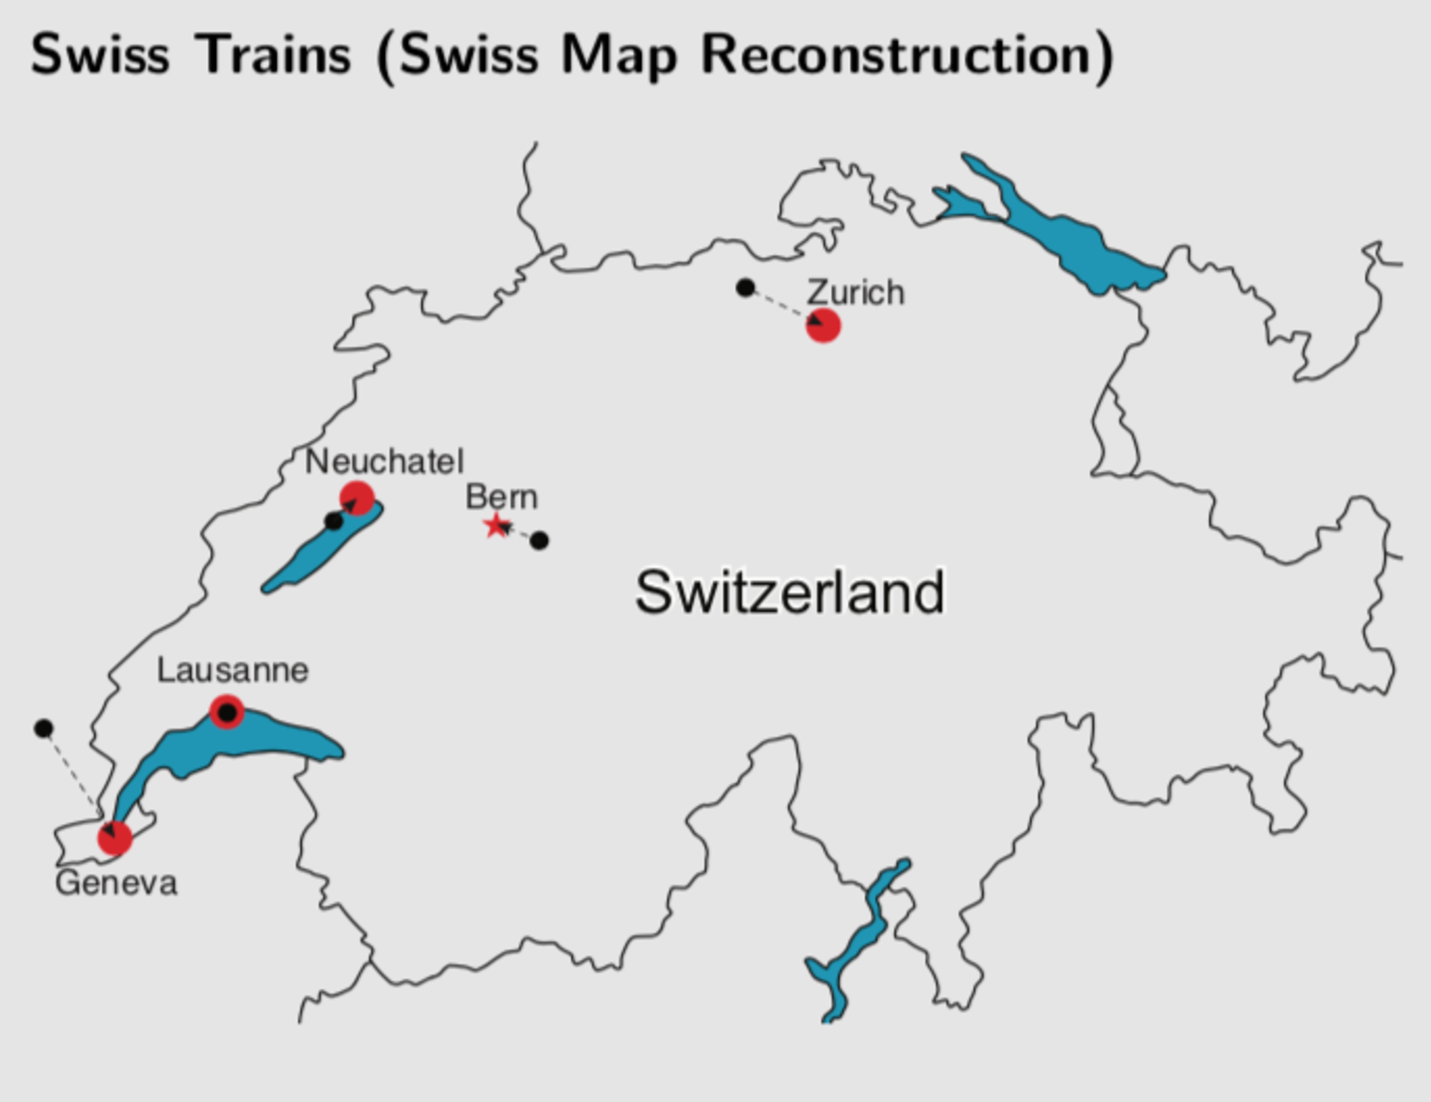
\includegraphics[width=0.4\textwidth]{images/swissEDM.pdf}
  \end{center}
  \caption{\footnotesize Image adapted from~\cite{dokmanic2015euclidean}. The red signs indicate the correct city locations. The black dots denote the recovered city locations.}
\end{wrapfigure}
% ---
\small  
In this toy problem, the authors aim at estimating the position of five cities on the Swiss map based not on the spatial distances between them, but on the time it takes to travel by train between them. Those time data (in minutes) are collected in the following timetable: \vspace{0.25cm}

%---
{\footnotesize\begin{blockarray}{cccccc}
& \text{L} & \text{G} & \text{Z} & \text{N} & \text{B} \\
\begin{block}{l(ccccc)}
  \text{Lausanne}  & 0   & 33  & 128 & 40 & 66 \\
  \text{Geneva}    & 33  & 0   & 158 & 64 & 101 \\
  \text{Zürich}    & 128 & 158 & 0   & 88 & 56 \\
  \text{Neuchâtel} & 40  & 64  & 88  & 0  & 34 \\
  \text{Bern}     & 66  & 101 & 56  & 34 & 0 \\
\end{block}\end{blockarray}.} \\

%---
Remarkably, even though these time data only roughly correlate with the physical distances between the cities, one can still obtain a remarkably good estimate of their positions on the Swiss map (up to some symmetries of the embedding space) using a multidimensional scaling algorithm.   
}}\normalsize \\
% ---------------------------------------------------

This example, if rather simple, nevertheless underlines well the key ingredients of methods that aim at retrieving points from distances that may not be directly measurable:
%---
\begin{enumerate}
    \item \textit{An appropriate proxy for the ``real'' distance}. In the above example, the proxy for the spatial distance between two cities is the time taken to travel by train between them. In our case, we shall consider the similarity between two projections to be a good proxy for their relative orientation.
    %
    \item \textit{A sufficiently rich collection of proxy distance data}. In this example, these data are provided by the (complete) train timetable. In our approach, we shall estimate the relative orientations between numerous pairs of projections based on the aforementioned proxy distance.  
    %
    \item \textit{An efficient recovery scheme}. In~\cite{dokmanic2015euclidean}, the embedding space being Euclidean, the theoretical framework of the Euclidean distance matrices (EDMs) guarantees that one can retrieve the desired points from the collected distances. In our case, as we shall shortly explain, we aim to embed the estimated relative orientations on $\SOThree$, the space of 3D rotations. Unfortunately, the extension of the EDM theory to such manifold is all but straightforward.
\end{enumerate}
%---

There is no simple way to ``handcraft'' a proxy distance that would robustly predict the similarity between two projections. Hence, we resort to \textit{learning} this distance function by parametrizing it as a neural network and capitalizing on 1) the public availability of large datasets of 3D atomic models\footnote{\texttt{https://www.ebi.ac.uk/pdbe/emdb}}, and 2) our ability to model the cryo-EM imaging process. This is the topic of Section~\ref{sec:estimating-relative-orientations}. 

Equipped with this learned distance, the idea is then to apply the aforementioned two-steps method (see Figure~\ref{fig:overview-pipeline}) for any projection dataset. As we just mentioned, we cannot rely on the theoretical framework of EDMs since our embedding space is non-Euclidean. Despite this lack of theoretical guarantees, we are able to appropriately minimize our objective function using a gradient-based algorithm, as we experimentally demonstrate in Section~\ref{sec:orientation-recovery}.

As a preamble, we discuss the need for a representation of orientations in $\SOThree$ that relies on unit quaternions. 
